\documentclass[conference]{IEEEtran}

\usepackage[UTF8,scheme=plain]{ctex}
\usepackage{amsmath,amssymb,amsfonts}
\usepackage{graphicx}
\usepackage{booktabs}
\usepackage{array}
\usepackage{multirow}
\usepackage{url}
\usepackage{xcolor}
\usepackage{microtype}
\usepackage[section]{placeins}

\graphicspath{{figures_paper/}{figures_cn/}{figures/}}

\title{RoadMC：面向路面病害分割的物理仿真点云生成与双阶段训练框架}

\author{\IEEEauthorblockN{YQGHL}
\IEEEauthorblockA{RoadMC repository snapshot\\
\texttt{https://github.com/YQGHL/roadmc}}}

\begin{document}
\maketitle

\begin{abstract}
路面病害点云分割面临标注稀缺、类别长尾、病害结构细薄以及真实采集成本高等问题。本文围绕 RoadMC 代码库给出一份中文 IEEE 风格报告，强调点云生成不是简单预处理，而是方法本身的一部分。RoadMC 先基于路面粗糙度谱、微纹理、病害几何原语和 LiDAR 观测模型合成带标签点云，再用统一的分割训练框架进行二分类稳定化与 38 类细分迁移。当前实验中，二分类最佳校准模型可达到 0.7319 的 mIoU、0.7052 的病害 IoU、0.9039 的精确率和 0.7624 的召回率；而 38 类短跑仍较不稳定，说明后续工作仍需继续强化数据规模、类别平衡和分阶段训练策略。
\end{abstract}

\begin{IEEEkeywords}
点云生成, 路面病害分割, Swin3D, PointMamba, mHC, Muon, 物理仿真
\end{IEEEkeywords}

\section{引言}
路面巡检是一个经典但并不轻松的感知任务。裂缝、坑槽、松散、沉陷和车辙等病害在几何上往往细长、稀疏、类别不平衡，而且真实标注非常昂贵。对于这类问题，合成点云的价值不只是“造数据”，更重要的是把几何先验、标签分布和采样方式都放进一个可控的监督闭环里。

RoadMC 的核心思路很简单：先生成，再学习，再校准。点云生成模块不是前处理脚本，而是方法主体的一部分，因为它直接决定几何形态、稀有病害覆盖率和标签分布上限；分割模型则负责验证这些合成数据到底能不能支撑有效训练。当前代码和实验都遵循一个稳定的路线，即先做二分类，再把二分类骨干迁移到 38 类细分任务。

本文的贡献可以概括为三点：
\begin{itemize}
  \item 给出一个物理仿真驱动的路面点云生成流程，覆盖路面先验、微纹理、病害原语和 LiDAR 观测模型；
  \item 给出一个模块化的点云分割框架，支持 Swin3D 或 PointMamba 骨干，支持 mHC 通道混合，并可切换 Muon/AdamW 优化策略；
  \item 基于项目日志总结当前最稳妥的实验路线：二分类稳定化、阈值校准、再迁移到 38 类细分。
\end{itemize}

\section{相关工作}
点云学习经历了从局部聚合到 Transformer，再到状态空间序列建模的演化。PointNet++ 通过分层局部特征学习奠定了点云任务的基础 \cite{pointnetpp}。Swin3D 将 Swin Transformer 的窗口注意力思想带入 3D 点云分析 \cite{swin3d}。PointMamba 则把状态空间建模引入点云场景，并以 Morton 顺序降低计算和存储开销 \cite{pointmamba}。

在长尾分割任务中，Focal Loss 仍然是处理背景压制和少数类稀缺的常用手段 \cite{focal}。而 mHC 则对应近期一种更稳定的超连接思路，它通过 Sinkhorn 归一化形成双随机通道混合矩阵，改善深层特征流动 \cite{mhc}。RoadMC 将这些思路组合为一个可切换、可消融、可迁移的工程化框架。

\section{方法}
\subsection{总体流程}
RoadMC 的端到端流程可以写成
\begin{equation}
S = \mathcal{G}(R, T, D, \mathcal{L}),
\end{equation}
其中 $R$ 表示路面粗糙度先验，$T$ 表示微纹理，$D$ 表示病害原语，$\mathcal{L}$ 表示 LiDAR 观测模型。生成的场景随后进入训练模块，形成“生成 - 训练 - 评估 - 校准”的闭环。

如图\ref{fig:overview}所示，总体方法不是简单地把点云预处理后丢给分割器，而是把合成模块作为监督数据来源的一部分。这样做的直接好处是：几何结构更可控，类别分布更可调，稀有病害的覆盖更容易做大。

\begin{figure*}[!t]
  \centering
  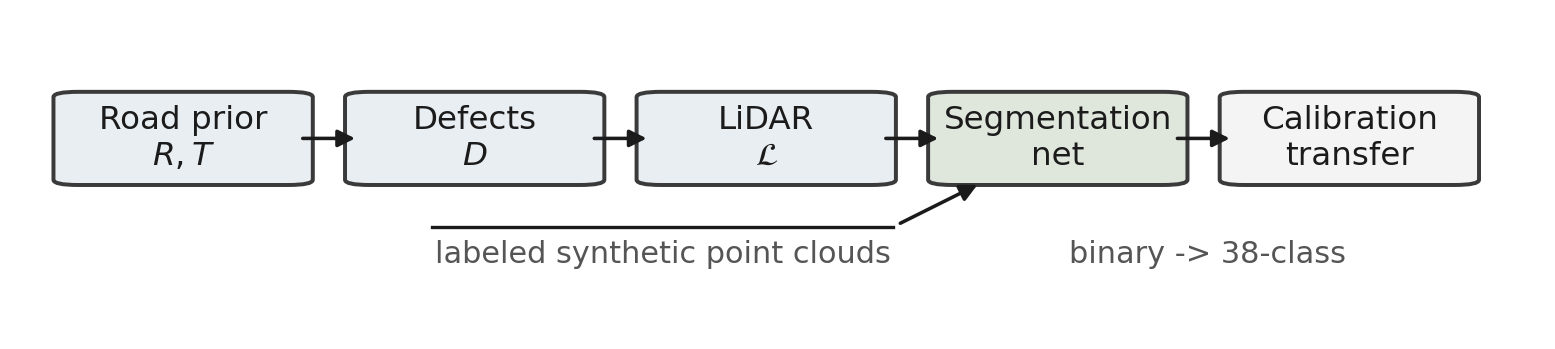
\includegraphics[width=0.78\textwidth]{roadmc_pipeline_compact.png}
  \caption{RoadMC 端到端框架。生成模块、分割网络与校准迁移构成闭环。}
  \label{fig:overview}
\end{figure*}

\subsection{点云生成模块}
RoadMC 的点云生成不是随机噪声叠加，而是“路面先验 + 病害形变 + 传感器观测”的合成链路。图\ref{fig:synthesis}给出了该模块的拆分。

\begin{figure}[!t]
  \centering
  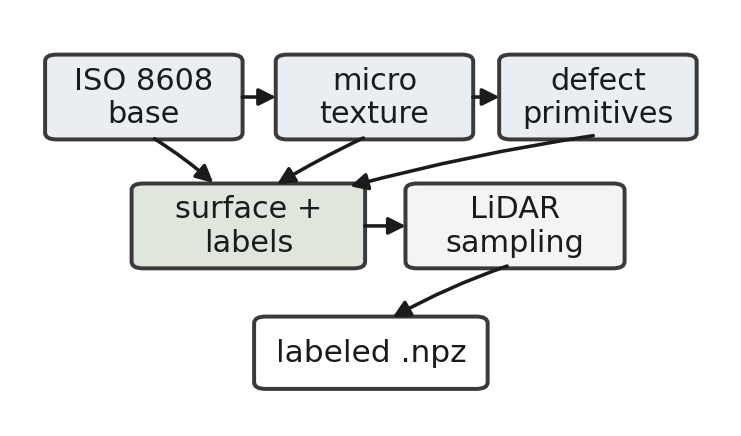
\includegraphics[width=0.88\columnwidth]{synthesis_compact.png}
  \caption{点云生成模块结构。}
  \label{fig:synthesis}
\end{figure}

首先，路面基底由 ISO 8608 粗糙度谱合成，使宏观表面具备合理的起伏统计。随后，微纹理通过分数布朗运动和局部曲率扰动叠加到表面上，从而避免“过于平滑”的合成痕迹。接着，病害原语在几何上生成裂缝、坑槽、松散、沉陷、车辙、波浪、剥落以及水泥路面常见病害，并把病害区域映射为点级标签。

更重要的是，LiDAR 观测模型不是附属项。它通过扫描线重采样、距离衰减、角度抖动和密度控制，把规则网格变成更接近真实扫描的非均匀点云。最后，场景被导出为包含 \texttt{points}、\texttt{labels}、\texttt{feats}、\texttt{normals} 和 \texttt{pavement\_type} 的压缩 \texttt{.npz} 文件，直接供训练使用。

\subsection{分割骨干与 mHC}
分割模块的输入接口是统一的：归一化 XYZ 坐标加上三维几何特征，即强度、曲率和裂缝边界距离。骨干网络可以在 Swin3D 与 PointMamba 之间切换，二者共享同一个解码头，便于做公平对比。图\ref{fig:backbone}给出了这一部分的结构。

\begin{figure}[!t]
  \centering
  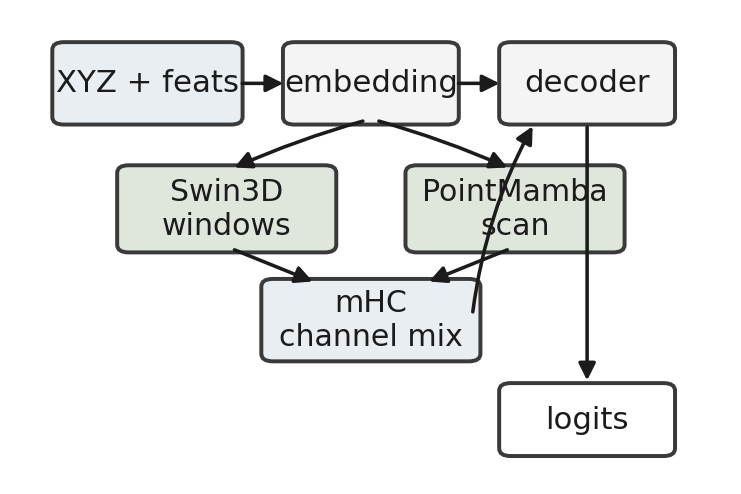
\includegraphics[width=0.88\columnwidth]{backbone_compact.png}
  \caption{分割骨干与 mHC 通道混合结构。}
  \label{fig:backbone}
\end{figure}

Swin3D 使用分层窗口注意力来聚合局部上下文，优势是表达能力强；PointMamba 则使用 Morton 顺序和扫描式状态更新，优势是轻量、速度快。mHC 在这里扮演通道混合器的角色，它不是必须项，但在当前代码中默认开启，便于测试残差通信是否有助于不同骨干。

解码头使用多尺度 skip fusion，把不同阶段的特征逐级融合到同一预测头中，输出逐点 logits。这样既保留浅层几何细节，也保留深层语义信息，比较适合路面这种细长目标与背景混杂的任务。

\subsection{训练、校准与迁移}
训练目标由三部分组成：
\begin{equation}
\mathcal{L} = \lambda_f \mathcal{L}_{\mathrm{focal}} + \lambda_d \mathcal{L}_{\mathrm{dice}} + \lambda_e \mathcal{L}_{\mathrm{edge}}.
\end{equation}
其中 Focal Loss 负责压制背景主导，Dice Loss 负责稳定小目标学习，Edge Loss 负责增强裂缝边界敏感性。图\ref{fig:training}把训练流程拆成了二分类优先、阈值校准、骨干迁移和 38 类细调四个阶段。

\begin{figure}[!t]
  \centering
  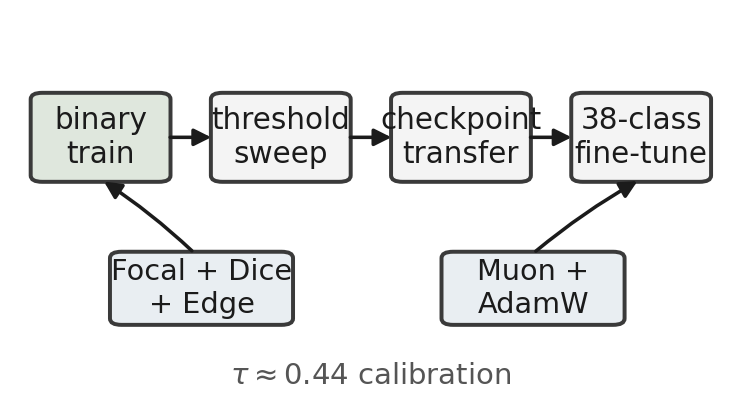
\includegraphics[width=0.88\columnwidth]{training_compact.png}
  \caption{二分类优先的训练、校准与迁移流程。}
  \label{fig:training}
\end{figure}

优化器采用 Muon/AdamW 混合策略：矩阵类参数交给 Muon，偏置、归一化等一维参数交给 AdamW。对于二分类验证，模型不直接使用 \texttt{argmax}，而是基于病害概率阈值 $\tau$ 做校准推理：
\begin{equation}
\hat{y}_i = \mathbb{1}\!\left[\mathrm{softmax}(z_i)_1 > \tau\right].
\end{equation}
当前项目日志表明，最佳阈值大约在 $0.44$ 附近。二分类阶段稳定后，再使用二分类 checkpoint 初始化骨干并继续训练 38 类头，是目前更合理的路线。

\section{实验设置}
当前报告主要基于合成二分类实验。默认配置如下：训练集 600 个场景，验证集 150 个场景，每个场景最多采样 512 个点，batch size 为 4，学习率为 $3\times 10^{-4}$，默认使用 mixed precision，二分类权重设置为 $\{1.0, 2.5\}$。

\begin{table}[t]
\centering
\caption{二分类实验的主要配置。}
\label{tab:setup}
\small
\begin{tabular}{p{0.34\columnwidth}p{0.56\columnwidth}}
\toprule
数据集 & 600 train / 150 val 合成场景 \\
输入点数 & 每个场景最多 512 点 \\
批大小 & 4 \\
优化器 & Muon，必要时回退 AdamW \\
骨干网络 & Swin3D 或 PointMamba \\
mHC & 默认开启 \\
二分类权重 & $\{1.0, 2.5\}$ \\
\bottomrule
\end{tabular}
\end{table}

\section{结果与分析}
表\ref{tab:results}汇总了当前最有代表性的二分类结果和一组轻量对比实验。最强的二分类模型来自 Swin3D + mHC，经过阈值校准后可达到 0.7319 的 mIoU。PointMamba 在短跑实验中速度更快，但精度仍略低于 Swin3D。

\begin{table*}[t]
\centering
\caption{合成验证集上的代表性结果与轻量对比。}
\label{tab:results}
\small
\setlength{\tabcolsep}{4pt}
\resizebox{\textwidth}{!}{%
\begin{tabular}{l l l l l}
\toprule
设置 & 协议 & 指标 & 数值 & 备注 \\
\midrule
Swin3D + mHC & 最佳校准 checkpoint & mIoU / disease IoU / precision / recall & 0.7319 / 0.7052 / 0.9039 / 0.7624 & 最优阈值约为 $\tau \approx 0.44$ \\
PointMamba + mHC & 200 step 二分类短跑 & final val mIoU / avg loss & 0.5671 / 0.8949 & 二分类权重 1.0 / 2.5 \\
Swin3D + mHC & 500 step 快速运行 & avg loss / elapsed & 3.7884 / 115.47 s & 训练更稳，但更慢 \\
PointMamba + mHC & 500 step 快速运行 & avg loss / elapsed & 4.0206 / 103.25 s & 更快，但 loss 略高 \\
\bottomrule
\end{tabular}%
}
\end{table*}

从项目日志看，二分类阶段已经具备可用性，尤其是在 class weight 和阈值校准到位之后，病害 IoU 不再是 0。相反，38 类短跑在当前配置下仍然容易退化到背景主导，或者只预测少数类别。换句话说，当前瓶颈并不是“模型完全不会学”，而是“长尾问题太强，训练阶段太短，监督粒度还不够稳”。

\FloatBarrier

\section{讨论}
这个项目最值得强调的一点，是生成器和分割器并不是前后两个无关步骤。生成器决定了几何先验、标签分布和稀有病害覆盖，分割器再反过来检验这些合成数据是否足够支撑学习。当前结果已经说明：二分类能先站稳，38 类才有继续往前走的基础。

下一步最自然的方向有三个。第一，把合成数据规模继续扩大到约 5000 个场景。第二，继续围绕二分类做阈值、权重和损失项的联合搜索，把 mIoU 往更高区间推。第三，在二分类骨干稳定后，再做 38 类的分阶段迁移，而不是直接从零硬训 38 类。

\section{结论}
RoadMC 把物理仿真点云生成和模块化点云分割串成了一个闭环。当前代码库已经形成了从路面先验合成、病害几何生成、LiDAR 观测仿真，到二分类稳定化、阈值校准和 38 类迁移的完整路径。就现阶段而言，最重要的结论不是“38 类已经完成”，而是“二分类已经足够稳，可以作为后续细分训练的坚实起点”。

\begin{thebibliography}{99}

\bibitem{pointnetpp}
C.~R. Qi, L. Yi, H. Su, and L.~J. Guibas, ``PointNet++: Deep hierarchical feature learning on point sets in a metric space,'' \emph{Advances in Neural Information Processing Systems}, vol.~30, 2017.

\bibitem{swin3d}
Y.-Q. Yang, Y.-X. Guo, and Y. Liu, ``Swin3D: A pretrained transformer backbone for 3D indoor scene understanding,'' \emph{arXiv preprint arXiv:2304.06906}, 2023.

\bibitem{pointmamba}
D. Liang \emph{et al.}, ``PointMamba: A simple state space model for point cloud analysis,'' \emph{arXiv preprint arXiv:2402.10739}, 2024.

\bibitem{mhc}
Z. Xie \emph{et al.}, ``mHC: Manifold-constrained hyper-connections,'' \emph{arXiv preprint arXiv:2512.24880}, 2025.

\bibitem{focal}
T.-Y. Lin \emph{et al.}, ``Focal loss for dense object detection,'' in \emph{Proc. IEEE Int. Conf. Computer Vision (ICCV)}, 2017, pp.~2980--2988.

\end{thebibliography}

\end{document}
